\section{Measurements}
\label{sec:meas}

During the final part of the course, electrical measurements were performed on the process control module (PCM) structures of the BICMOS5 wafer: Van der Pauw (VdP) squares, electrical line width measurement (ELM) resistors, and NMOS/PMOS transistors in all four $V_\mathrm{T}$-adjust quadrants. These measurements close the loop of the course: they are compared with the analytical calculations of Section~\ref{sec:tech}, the simulations of Sections~\ref{sec:procsim} and~\ref{sec:devsim}, and the in-line processing measurements of Section~\ref{sec:processing}.

The measurements were taken on a Cascade 31 automatic probe station with a Keysight B1500A parameter analyzer controlled by IC-CAP, using four-point probing throughout, so that probe and contact resistances drop out of the results. Following the course guidelines, no IC-CAP screenshots are used here: all raw data were exported and re-plotted in MATLAB.

The junction depths $x_\mathrm{j}$ of the N-Well, SN and SP implants were taken from the Sentaurus simulations in Section~\ref{sec:devsim}, and the in-line sheet resistances from Section~\ref{sec:processing}, so the measurements here can be compared directly with the earlier process and simulation results.

\subsection{The BICMOS5 Test Wafer}

The course wafer is a $10$ cm wafer processed at the Else Kooi Laboratory, containing over 160 dies of $6\times6$ mm \cite{et4icp_manual}. The wafer is divided into four quarters, each of which received a different boron $V_\mathrm{T}$-adjust dose during processing: $0$ (top left), $3\times10^{11}$ (bottom left), $6\times10^{11}$ (top right) and $9\times10^{11}\,\mathrm{cm}^{-2}$ (bottom right), as shown in Figure~\ref{fig:wafer-layout}(a). Measuring the same device type in each quarter therefore reveals the influence of the $V_\mathrm{T}$-adjust dose directly.

Each die (Figure~\ref{fig:wafer-layout}(b)) contains several blocks, of which four are used in this course: a PMOS transistor block and an NMOS transistor block with various gate geometries, a block of Van der Pauw structures, and the electrical linewidth measurement structures. The resistive structures are strips implanted into a region of the opposite doping type, so each strip is isolated from its surroundings by a pn-junction; this isolation only holds as long as that junction stays reverse biased, a condition that returns in the choice of the measurement voltages below.

\begin{figure}[H]
  \centering
  \begin{subfigure}{0.42\textwidth}
    \centering
    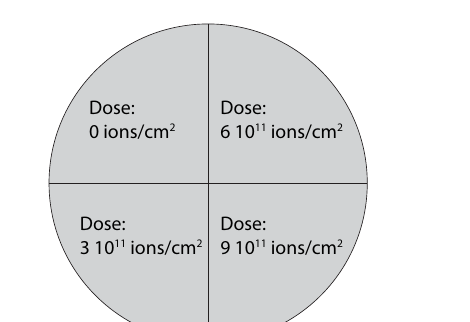
\includegraphics[width=0.85\linewidth]{Figures/fig5-2_vt_adjust_quarters.png}
    \caption{$V_\mathrm{T}$-adjust doses per wafer quarter.}
    \label{fig:wafer-quadrants}
  \end{subfigure}
  \hfill
  \begin{subfigure}{0.55\textwidth}
    \centering
    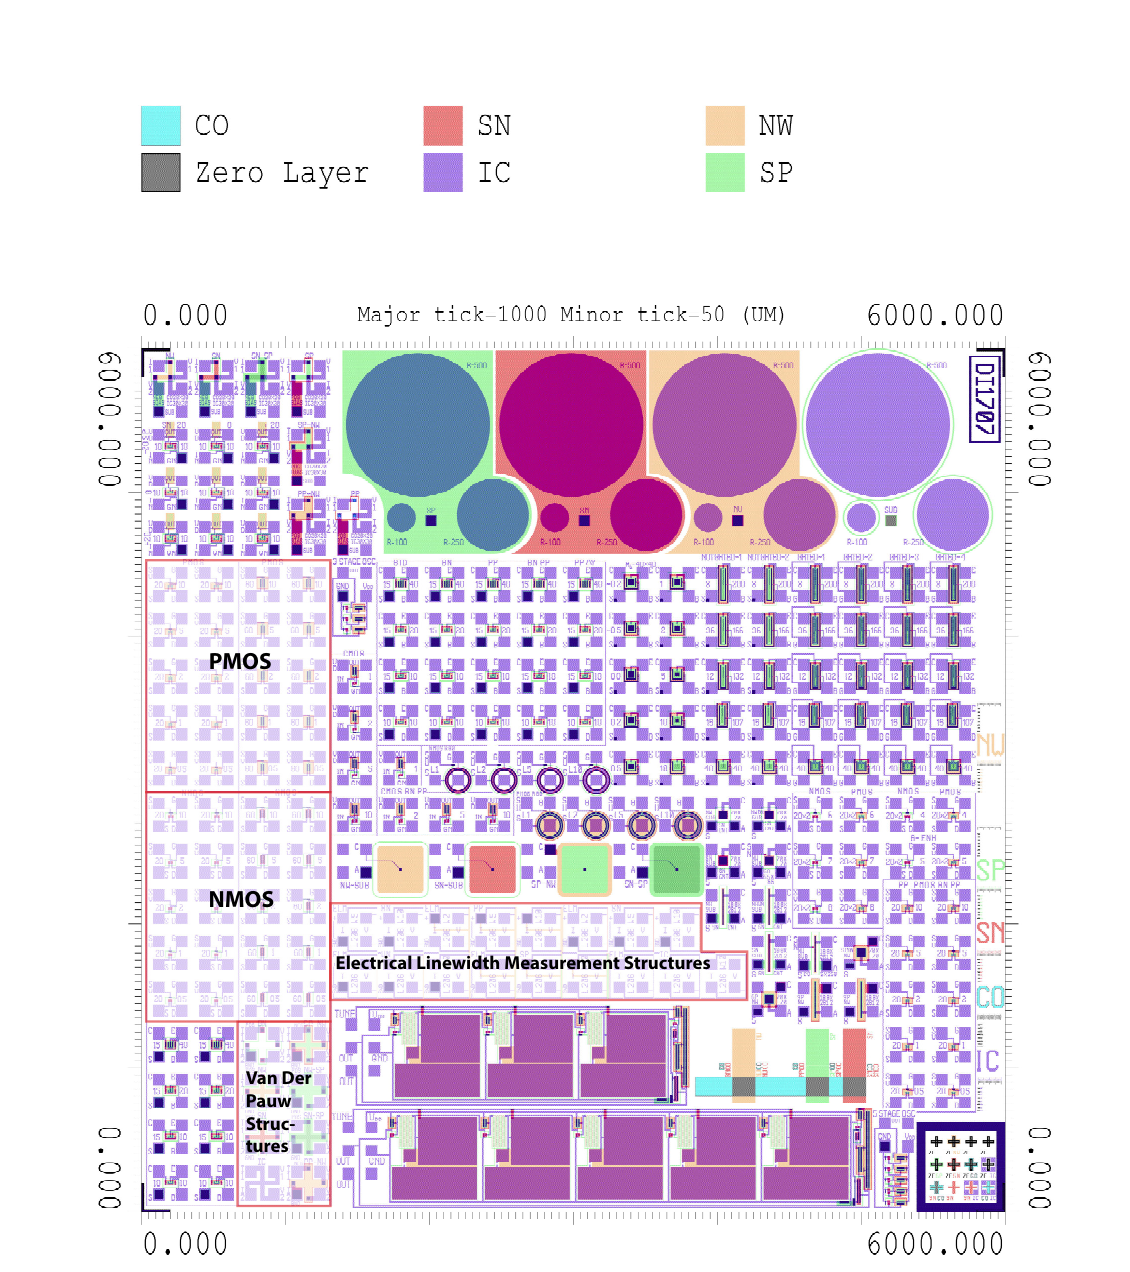
\includegraphics[width=0.95\linewidth]{Figures/fig5-3_die_layout.png}
    \caption{Layout of one $6000\times6000\,\mu$m die; each colour is a mask.}
    \label{fig:die-layout}
  \end{subfigure}
  \caption{The BICMOS5 test wafer: (a) the four $V_\mathrm{T}$-adjust quarters and (b) the die layout with the PMOS, NMOS, ELM and Van der Pauw blocks used in this course \cite{et4icp_manual}.}
  \label{fig:wafer-layout}
\end{figure}

\subsection{Van der Pauw Sheet Resistance and Doping Concentration}

The sheet resistance $R_\mathrm{s} = \rho/d$ of a layer with resistivity $\rho$ and thickness $d$ allows a designer to compute the resistance of any strip of that layer as $R = R_\mathrm{s} L/W$, with $L$ the strip length and $W$ its width. The Van der Pauw structures on the die are greek crosses: a $30\times30\,\mu$m square of the layer to be measured with a contact on each side, drawn for each implantation and layer combination (Figure~\ref{fig:vdp-structures}). The VdP structures were measured in the top-left quadrant ($V_\mathrm{T}$-adjust dose $0$) using a symmetric four-point configuration. The analyzer swept the force voltage between $-0.2$\,V and $+0.2$\,V at grounded substrate, and the resistance $R_{AB,CD}$ was obtained from the least-squares slope of the sensed voltage difference $V_1 - V_2$ versus the forced current $I_\mathrm{force}$. For a symmetric VdP structure a single measurement suffices, and the sheet resistance follows from the Van der Pauw relation \cite{vanderpauw1958method}
\begin{equation}
  R_\mathrm{s} = \frac{\pi}{\ln 2}\, R_{AB,CD} \approx 4.532\, R_{AB,CD},
  \label{eq:vdp}
\end{equation}
where $R_{AB,CD}$ is the resistance measured by forcing a current through contacts A and B and sensing the voltage over contacts C and D, and the factor $\pi/\ln 2$ corrects for the radial current flow in the square structure.

\begin{figure}[H]
  \centering
  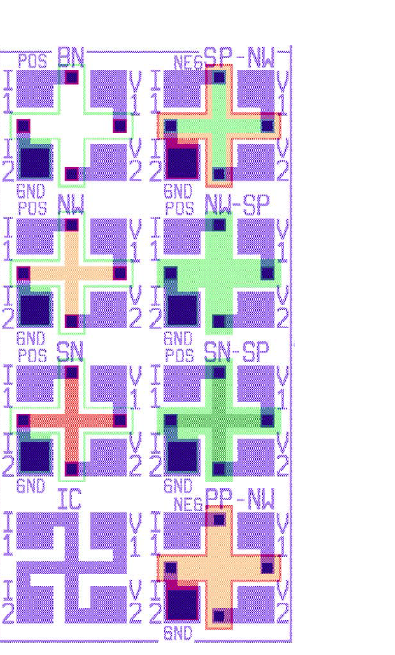
\includegraphics[width=0.35\linewidth]{Figures/fig5-5_van_der_pauw.png}
  \caption{Greek-cross Van der Pauw structures for the different layers and layer combinations, with the current (I) and voltage (V) probe pads indicated \cite{et4icp_manual}.}
  \label{fig:vdp-structures}
\end{figure}

The small sweep range is essential: the implanted layers form pn-junctions with the substrate (or well) underneath, and a silicon junction only conducts appreciably above its exponential knee of about $0.6$\,V. Within $\pm 0.2$\,V the junction current is orders of magnitude below the lateral sheet current for either sweep polarity, so the carriers stay confined in the implanted layer, as the VdP method requires. At larger voltages the forward-biased half of the sweep would open the junction and current would spread through the entire substrate, collapsing the measured resistance.

The measured I/V sweeps and their linear fits are shown in Figure~\ref{fig:vdp-fits}; the extracted values are summarized in Table~\ref{tab:ch6-vdp-rsheet}. The last column repeats the in-line monitor values from Section~\ref{sec:processing} for comparison.

\begin{figure}[H]
  \centering
  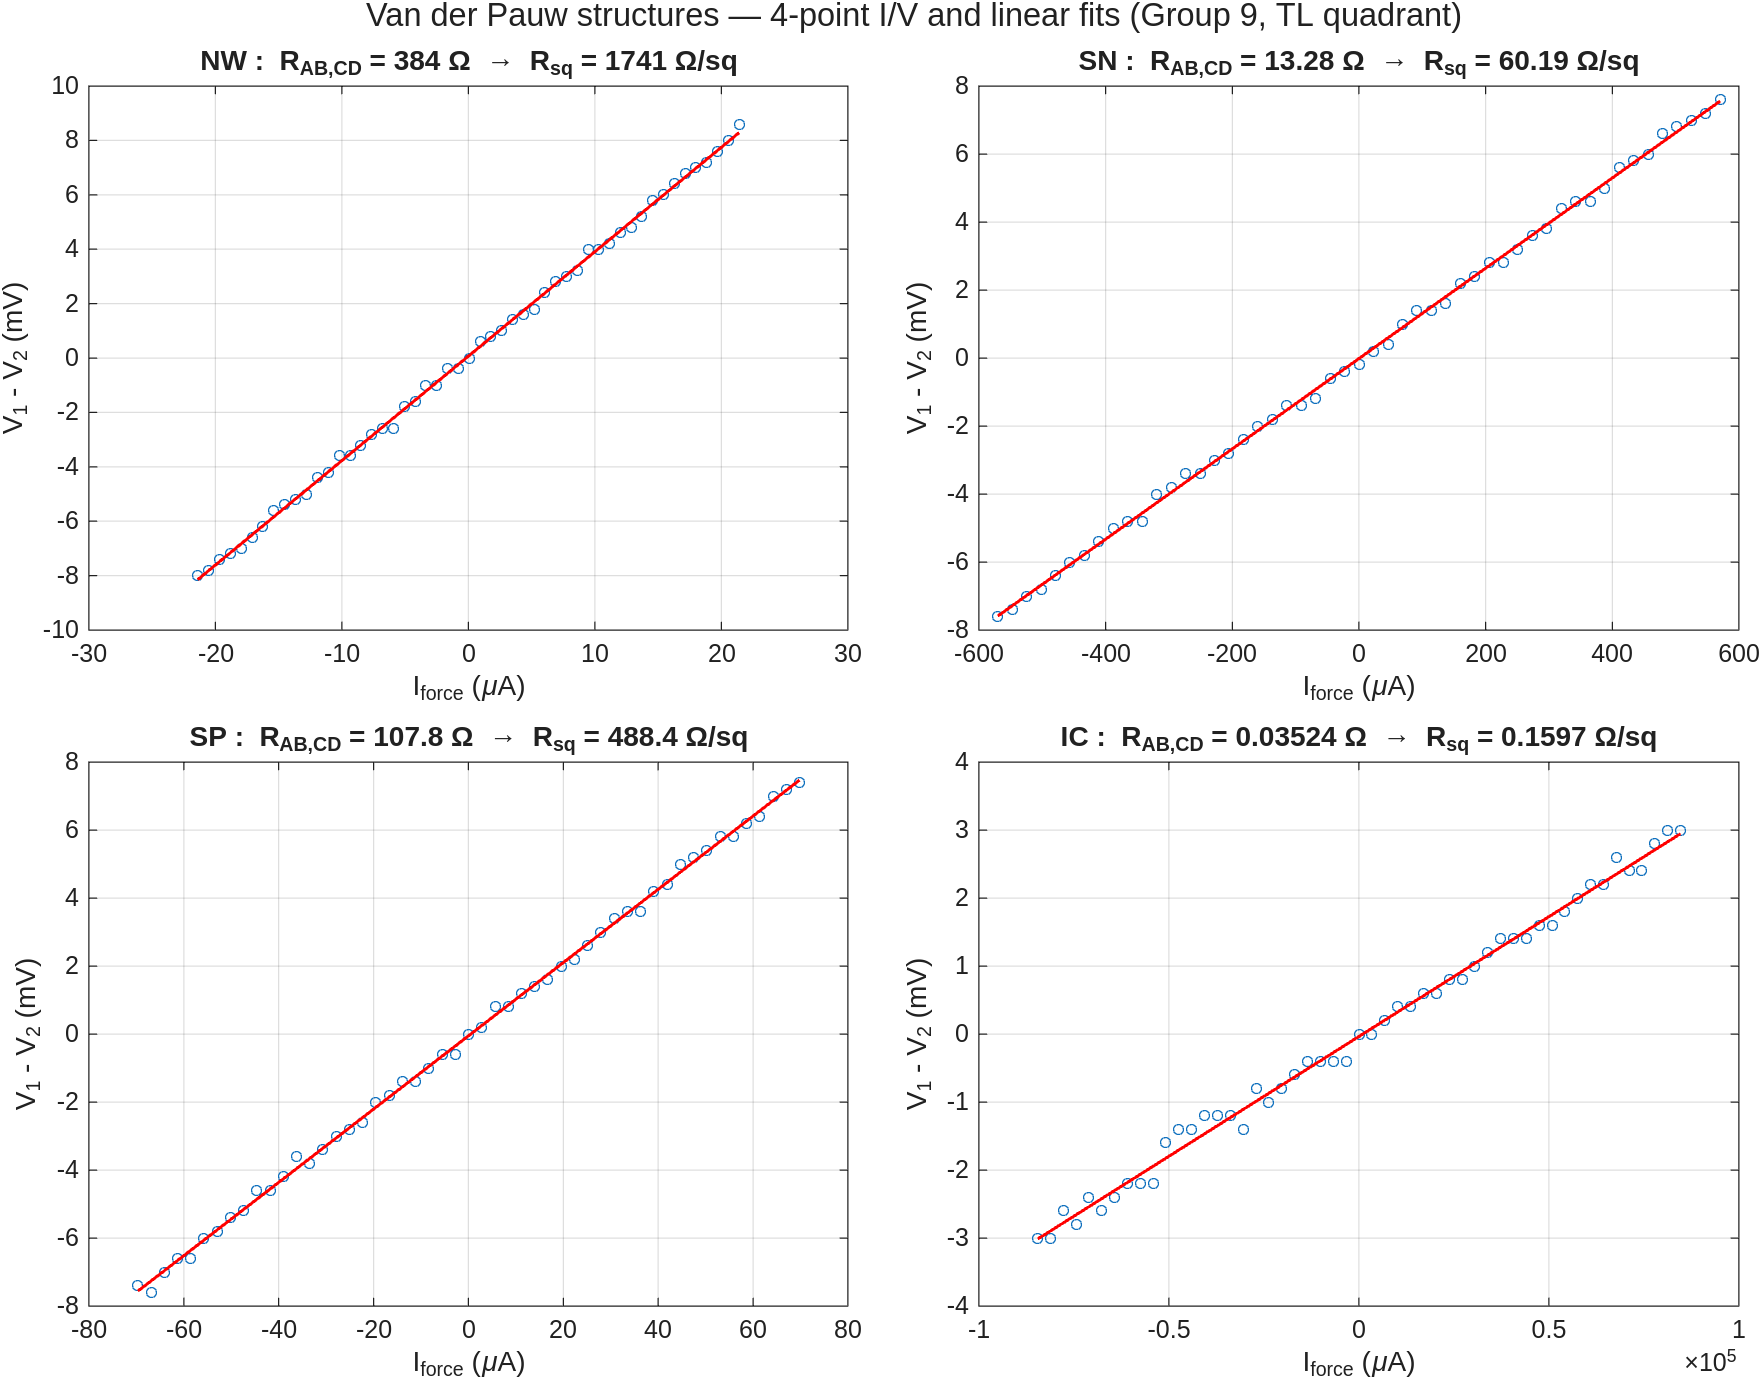
\includegraphics[width=0.95\linewidth]{Figures/vdp_iv_fits.png}
  \caption{Van der Pauw four-point I/V sweeps and linear fits for the N-Well, SN, SP and IC (metal) layers, measured in the top-left quadrant. All fits have $R^2 > 0.99$.}
  \label{fig:vdp-fits}
\end{figure}

\begin{table}[htbp]
  \centering
  \caption{Van der Pauw sheet resistances of the implanted layers and metal, compared to the in-line monitor values from Section~\ref{sec:processing}.}
  \label{tab:ch6-vdp-rsheet}
  \begin{tabular}{lrrrr}
    \toprule
    Layer & $R_{AB,CD}$ ($\Omega$) & $R_\mathrm{s}$ ($\Omega/\square$) & Fit $R^2$ & In-line $R_\mathrm{s}$ ($\Omega/\square$) \\
    \midrule
    N-Well      & 384.02  & 1740.5 & 0.9991 & 1488.8 \\
    SN          &  13.28  &   60.19 & 0.9991 &   57.4 \\
    SP (in N-Well) & 107.75 & 488.4 & 0.9990 & 510.6 \\
    IC metal    &   0.0352 & 0.160 & 0.9939 & -- \\
    \bottomrule
  \end{tabular}
\end{table}

The SN and SP values agree with the in-line monitor resistances to within about $5\%$, while the N-Well shows a larger deviation of roughly $17\%$. This is consistent with the N-Well being the most lightly doped layer, and therefore the most sensitive to wafer position, surface depletion, and the difference between the blanket monitor wafer used in the cleanroom and the drawn VdP cloverleaf on the PCM.

The IC metal has a sheet resistance of only $0.160\,\Omega/\square$, three to four orders of magnitude lower than the implanted silicon layers, whose values range from about $60\,\Omega/\square$ for SN to $1740\,\Omega/\square$ for the N-Well. With the known film thickness $d = 0.2\,\mu\mathrm{m}$, the metal resistivity follows as $\rho = R_\mathrm{s}\,d = 3.2\times10^{-6}\,\Omega\,\mathrm{cm}$, which matches the literature value for Al with $1\%$ Si. The root cause of the difference in magnitude is the free-carrier density: aluminium contains roughly one conduction electron per atom (about $10^{23}\,\mathrm{cm}^{-3}$), whereas the implanted layers only contain $10^{16}$ to $10^{19}\,\mathrm{cm}^{-3}$ activated dopants. The higher carrier mobility in lightly doped silicon only partly offsets this. For this reason the metal layer is used for low-resistance interconnects, while the implanted layers are suitable for making resistors.

Using the simulated junction depths $x_\mathrm{j}$ from Section~\ref{sec:devsim}, the depth-averaged resistivity of each implanted layer follows from
\begin{equation}
  \rho = R_\mathrm{s}\,x_\mathrm{j}.
  \label{eq:rho-vdp}
\end{equation}
The average active dopant concentration $\bar N$ is then obtained from the Irvin curves for the corresponding carrier type, here evaluated with the Masetti doping-dependent mobility model \cite{masetti1983modeling}. The resulting resistivities and concentrations are given in Table~\ref{tab:ch6-vdp-conc}.

\begin{table}[htbp]
  \centering
  \caption{Depth-averaged resistivity and active dopant concentration from the VdP measurements and Irvin curves, compared to the values from Section~\ref{sec:processing}.}
  \label{tab:ch6-vdp-conc}
  \begin{tabular}{lccccc}
    \toprule
    Layer & $x_\mathrm{j}$ ($\mu$m) & $\rho = R_\mathrm{s}x_\mathrm{j}$ ($\Omega\,\mathrm{cm}$) & Type & $\bar N$ ($\mathrm{cm}^{-3}$) & Sec.~\ref{sec:processing} $N$ ($\mathrm{cm}^{-3}$)\\
    \midrule
    N-Well & 2.085 & 0.363            & n & $1.5\times10^{16}$ & $1.5\times10^{16}$ \\
    SN     & 0.537 & $3.2\times10^{-3}$ & n & $2.3\times10^{19}$ & $2\times10^{19}$ \\
    SP     & 0.594 & $2.9\times10^{-2}$ & p & $1.6\times10^{18}$ & $1.5\times10^{18}$ \\
    \bottomrule
  \end{tabular}
\end{table}

The doping concentrations obtained from the three routes are therefore consistent within their meaning. The VdP and in-line values agree to within about $10\%$ for all three layers, which is remarkable for two independent electrical measurements on different structures. Compared to the simulations of Section~\ref{sec:procsim}, the extracted values are depth-averaged active concentrations: for the steep, solid-solubility-limited SN profile the average sits roughly an order of magnitude below the simulated peak of $1.8\times10^{20}\,\mathrm{cm}^{-3}$, while for the flatter N-Well and SP profiles the average is close to the simulated levels. It should also be noted that the measured sheet resistances are only consistent with the simulated junction depths: inserting the much shallower analytical depths of Section~\ref{sec:tech} into Equation~\eqref{eq:rho-vdp} would produce unphysical concentrations, which confirms that the analytical model misses the thermal budget of the real process.

\subsection{Electrical Line Width Measurements and Lateral Out-Diffusion}

During the anneals, dopant atoms not only diffuse deeper into the silicon but also sideways out of the implantation window, so a resistor line is electrically wider than drawn. To probe this lateral out-diffusion, ELM structures with drawn widths $W = 2$, $5$ and $10\,\mu\mathrm{m}$ and length $L = 206\,\mu\mathrm{m}$ were measured for the N-Well and SN implants. Each ELM structure is a differential resistor with four contacts (Figure~\ref{fig:elm-structures}): the outermost contacts force a current through the strip, and two inner contacts sense the voltage drop over the $206\,\mu\mathrm{m}$ length, so the measurement is again free of contact resistance. For each resistor a four-point measurement was taken and the apparent sheet resistance was computed as
\begin{equation}
  R_\mathrm{s,app} = R\, \frac{W}{L},
  \label{eq:elm-app}
\end{equation}
using the drawn width $W$. The results are listed in Table~\ref{tab:ch6-elm-raw} and plotted against the drawn width in Figure~\ref{fig:elm-rsq}.

\begin{figure}[H]
  \centering
  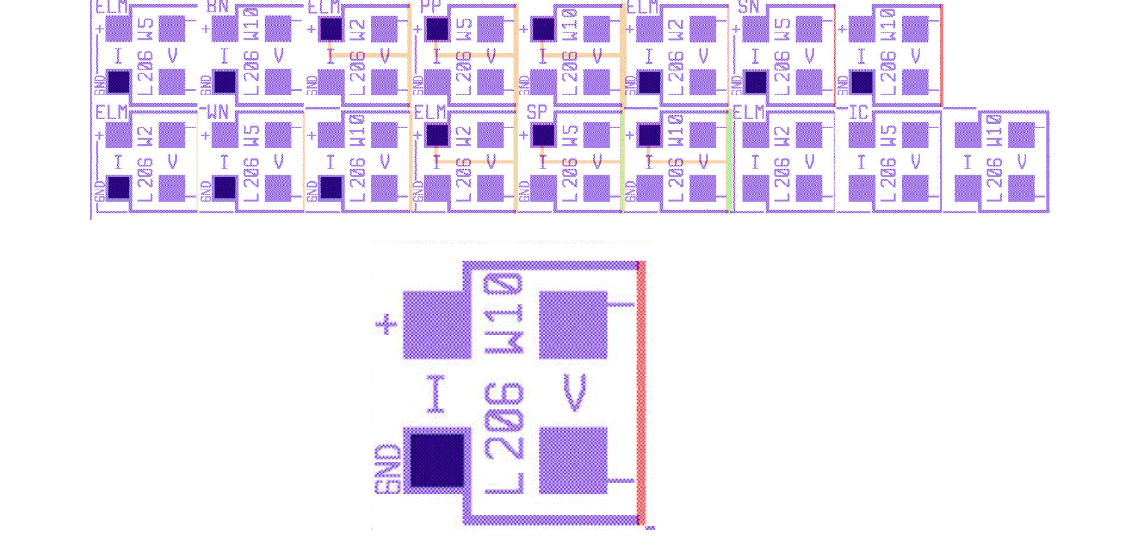
\includegraphics[width=0.95\linewidth]{Figures/fig_elm_structures.png}
  \caption{The ELM block with the differential resistors of all layers (top) and the detailed view of one structure (bottom). The two capital letters give the mask (e.g.\ SN), the number after W the drawn line width in $\mu$m; all strips have $L = 206\,\mu$m \cite{et4icp_manual}.}
  \label{fig:elm-structures}
\end{figure}

\begin{table}[htbp]
  \centering
  \caption{Raw ELM resistances and apparent sheet resistances for N-Well and SN resistors ($L = 206\,\mu\mathrm{m}$).}
  \label{tab:ch6-elm-raw}
  \begin{tabular}{lrrr}
    \toprule
    Layer & $W$ ($\mu$m) & $R$ ($\Omega$) & $R_\mathrm{s,app}$ ($\Omega/\square$) \\
    \midrule
    N-Well &  2 & 58832.7 & 571.2 \\
    N-Well &  5 & 38478.1 & 933.9 \\
    N-Well & 10 & 19689.2 & 955.8 \\
    SN     &  2 &  5244.8 &  50.9 \\
    SN     &  5 &  2273.5 &  55.2 \\
    SN     & 10 &  1171.1 &  56.8 \\
    \bottomrule
  \end{tabular}
\end{table}

\begin{figure}[H]
  \centering
  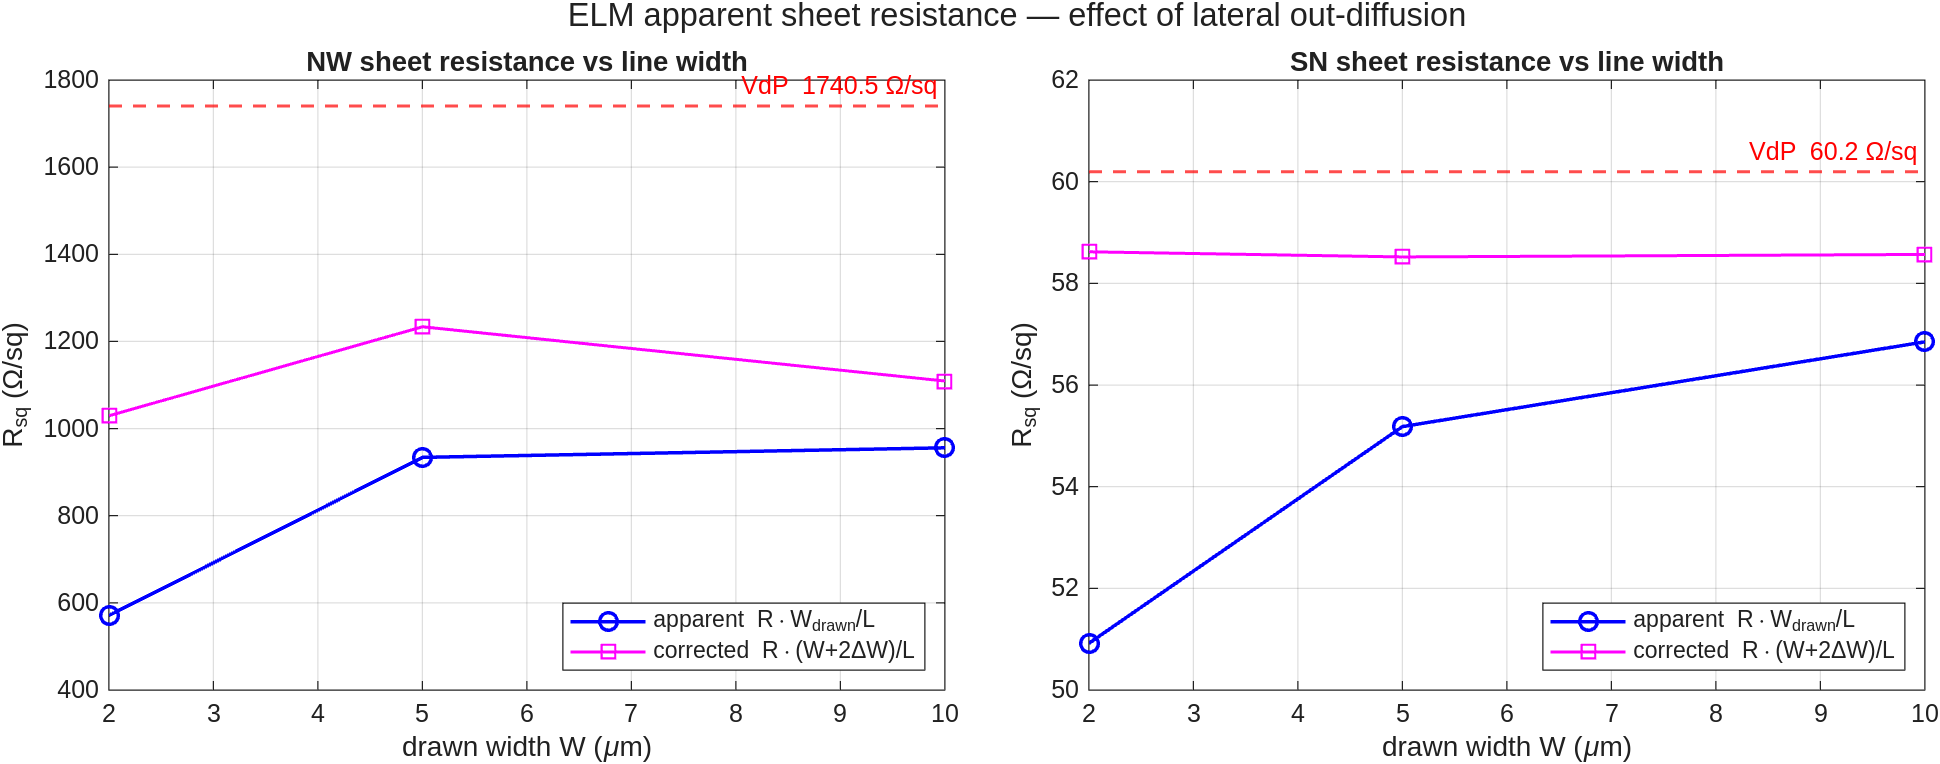
\includegraphics[width=0.9\linewidth]{Figures/elm_rsq_vs_width.png}
  \caption{Apparent ELM sheet resistance versus drawn line width for the N-Well and SN implants. The dashed lines indicate the Van der Pauw reference values.}
  \label{fig:elm-rsq}
\end{figure}

For both implants the apparent sheet resistance computed with the drawn width is systematically lower than the VdP value, and the deficit grows as the line becomes narrower ($-67\%$ for the $2\,\mu\mathrm{m}$ N-Well line versus $-15\%$ for the $2\,\mu\mathrm{m}$ SN line). This shows that the conducting strip is wider than its nominal geometry because of lateral dopant diffusion; a fixed widening matters relatively more for narrow lines. The effective width can be written as
\begin{equation}
  W_\mathrm{eff} = W + 2\Delta W,
  \label{eq:weff}
\end{equation}
where $\Delta W$ is the lateral out-diffusion per side.

Assuming a constant $\Delta W$, the conductance is linear in the drawn width, $1/R = (W + 2\Delta W)/(R_\mathrm{s} L)$, so a straight-line fit of $1/R$ versus $W$ yields the true sheet resistance from the slope and $\Delta W$ from the intercept. The fits are shown in Figure~\ref{fig:elm-dw} and the extracted values are summarized in Table~\ref{tab:ch6-elm-fit}.

\begin{figure}[H]
  \centering
  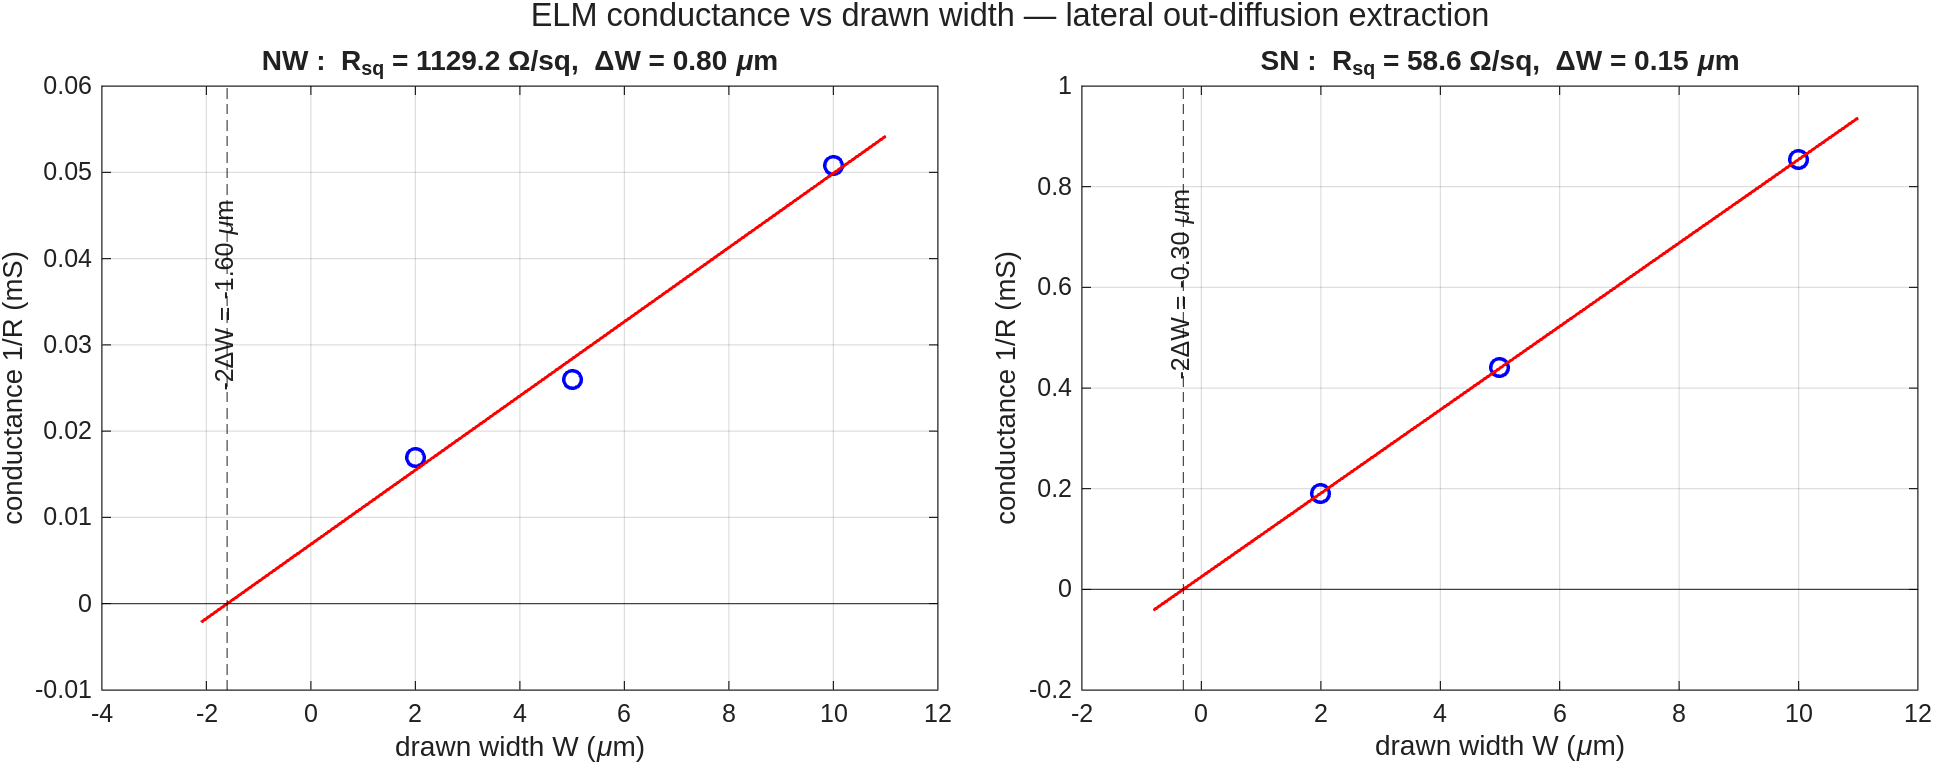
\includegraphics[width=0.9\linewidth]{Figures/elm_deltaW_fit.png}
  \caption{ELM conductance versus drawn width with linear fits. The extrapolation to zero conductance yields the lateral out-diffusion $\Delta W$ per side.}
  \label{fig:elm-dw}
\end{figure}

\begin{table}[htbp]
  \centering
  \caption{Sheet resistance and lateral out-diffusion extracted from the ELM structures.}
  \label{tab:ch6-elm-fit}
  \begin{tabular}{lrrr}
    \toprule
    Layer & $R_\mathrm{s,ELM}$ ($\Omega/\square$) & $\Delta W$ ($\mu$m) & Fit $R^2$ \\
    \midrule
    N-Well & 1129.2 & 0.80 & 0.986 \\
    SN     &   58.6 & 0.15 & 0.999999 \\
    \bottomrule
  \end{tabular}
\end{table}

For the SN implant the extraction is textbook-like: the conductance is perfectly linear in width, the ELM sheet resistance agrees with the VdP value ($60.2\,\Omega/\square$) to within about $3\%$, and the extracted lateral out-diffusion is only $\Delta W \approx 0.15\,\mu\mathrm{m}$ per side. The N-Well behaves differently: the three points are not exactly collinear and the free fit returns a sheet resistance well below the VdP value. Anchoring the sheet resistance to the VdP value ($1740\,\Omega/\square$) instead, the narrow lines consistently indicate an out-diffusion closer to $2.1\,\mu\mathrm{m}$ per side, comparable to the vertical junction depth. The constant-$\Delta W$ model is simply too crude for the N-Well, whose laterally diffused edges are graded over about $2\,\mu\mathrm{m}$, so each line width samples a different effective sheet resistance.

The large difference in out-diffusion between the two implants has two causes. First, the thermal budget: the N-Well phosphorus receives a $4$\,h drive-in at $1150\,^\circ$C, which is what makes it $2\,\mu\mathrm{m}$ deep, and diffusion is isotropic, so the dopant spreads sideways by a comparable amount. The SN arsenic only sees the much shorter gate-oxidation anneal. Second, the species: arsenic diffuses roughly an order of magnitude slower than phosphorus at the same temperature. Both effects together explain why $\Delta W$ for the N-Well is more than five times the SN value.

\subsection[Transistor Characterisation]{Transistor Characterisation: Threshold, Mobility, Short-Channel Effects}

The PMOS and NMOS blocks of the die each contain 20 transistors with different combinations of the two gate dimensions, labelled in the layout by the device type letter with the two dimensions in $\mu$m next to it (Figure~\ref{fig:mos-blocks}). NMOS and PMOS transistors with gate geometries $W\!:\!L = 20\!:\!1$, $20\!:\!2$, $20\!:\!5$, $20\!:\!10$ and $60\!:\!2$ (gate width : gate length, in $\mu\mathrm{m}$) were measured in the bottom-right quadrant ($V_\mathrm{T}$-adjust dose $9\times10^{11}\,\mathrm{cm}^{-2}$). Transfer characteristics $I_\mathrm{D}(V_\mathrm{G})$ were recorded at $|V_\mathrm{D}| = 0.1$\,V and threshold voltages and mobilities were extracted using the long-channel unified model. In the linear region ($|V_\mathrm{DS}|$ small) the drain current is
\begin{equation}
  I_\mathrm{D} = \mu\, C_\mathrm{ox} \frac{W}{L} \left( V_\mathrm{GS} - V_\mathrm{T} - \frac{V_\mathrm{DS}}{2} \right) V_\mathrm{DS},
  \label{eq:idlin}
\end{equation}
where $\mu$ is the carrier mobility, $C_\mathrm{ox} = \varepsilon_0\varepsilon_\mathrm{SiO_2}/t_\mathrm{ox} = 3.45\times10^{-8}\,\mathrm{F/cm^2}$ the oxide capacitance per unit area for the $t_\mathrm{ox} = 100$\,nm gate oxide, $W$ and $L$ the gate width and length, and $V_\mathrm{GS}$, $V_\mathrm{DS}$ and $V_\mathrm{T}$ the gate-source, drain-source and threshold voltages. The threshold voltage was extracted by linear extrapolation of $I_\mathrm{D}(V_\mathrm{G})$ at the point of maximum transconductance $g_\mathrm{m,max}$ (corrected by $V_\mathrm{DS}/2$), and the mobility follows from the transconductance as
\begin{equation}
  \mu = \frac{g_\mathrm{m,max}\,L}{C_\mathrm{ox}\,W\,|V_\mathrm{DS}|}.
  \label{eq:mob}
\end{equation}

\begin{figure}[H]
  \centering
  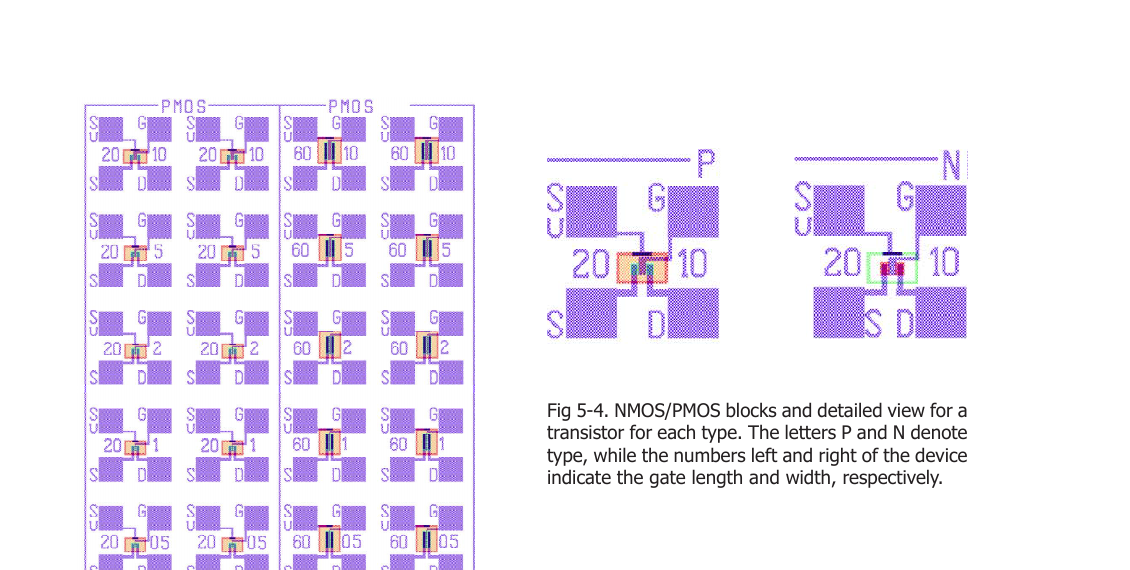
\includegraphics[width=0.75\linewidth]{Figures/fig5-4_nmos_pmos_blocks.png}
  \caption{Part of the PMOS transistor block and the detailed view of one PMOS and one NMOS device with their source (S), gate (G), drain (D) and substrate (SU) pads; the numbers next to each device give its gate dimensions in $\mu$m \cite{et4icp_manual}.}
  \label{fig:mos-blocks}
\end{figure}

Figure~\ref{fig:idvg-geoms} shows the measured transfer characteristics of all geometries; the extracted parameters are listed in Table~\ref{tab:ch6-transfers}.

\begin{figure}[H]
  \centering
  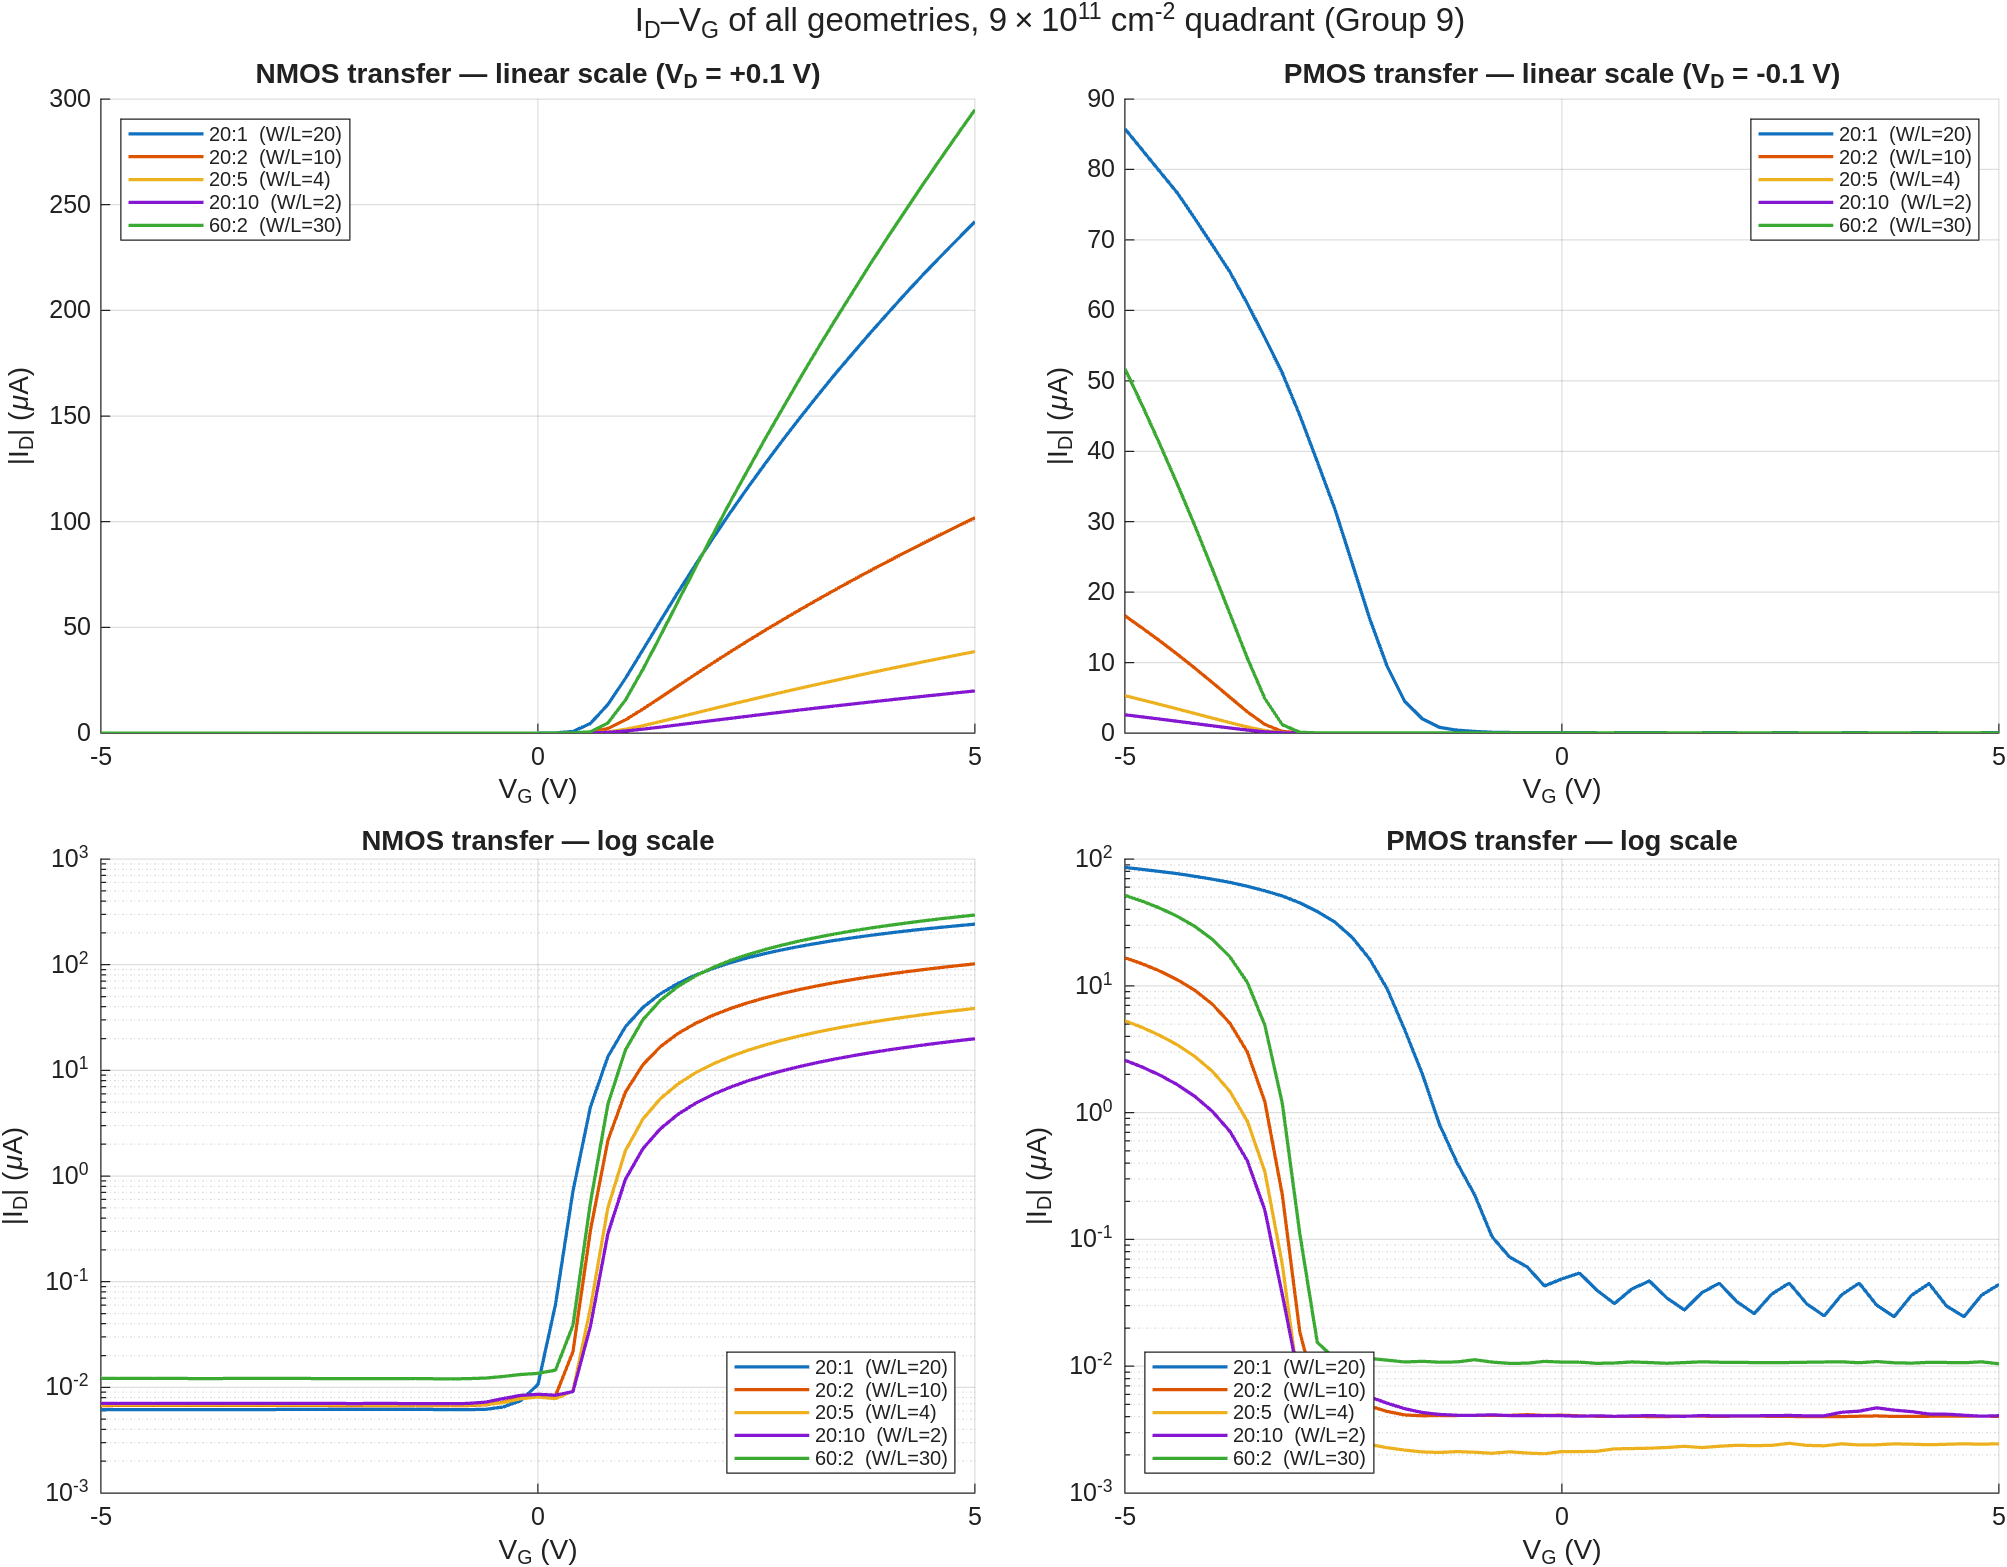
\includegraphics[width=0.95\linewidth]{Figures/idvg_geometries.png}
  \caption{Measured NMOS and PMOS transfer characteristics for all gate geometries at $|V_\mathrm{D}| = 0.1$\,V in the $9\times10^{11}\,\mathrm{cm}^{-2}$ quadrant, on linear and logarithmic current scales.}
  \label{fig:idvg-geoms}
\end{figure}

\begin{table}[htbp]
  \centering
  \caption{Threshold voltages and mobilities extracted from the transfer characteristics in the $9\times10^{11}\,\mathrm{cm}^{-2}$ quadrant ($V_\mathrm{D} = \pm 0.1$\,V).}
  \label{tab:ch6-transfers}
  \begin{tabular}{lrrrr}
    \toprule
    Type & $W\!:\!L$ & $V_\mathrm{T}$ (V) & $g_\mathrm{m,max}$ ($\mu$S) & $\mu$ ($\mathrm{cm}^2/\mathrm{V\,s}$) \\
    \midrule
    NMOS & 20:1  &  0.572 & 68.0  & 985 \\
    NMOS & 20:2  &  0.740 & 27.5  & 796 \\
    NMOS & 20:5  &  0.819 & 10.1  & 734 \\
    NMOS & 20:10 &  0.811 & 5.18  & 750 \\
    NMOS & 60:2  &  0.779 & 80.6  & 778 \\
    \midrule
    PMOS & 20:1  & -1.733 & 39.0  & 565 \\
    PMOS & 20:2  & -3.262 & 10.4  & 301 \\
    PMOS & 20:5  & -3.300 & 3.25  & 236 \\
    PMOS & 20:10 & -3.305 & 1.59  & 230 \\
    PMOS & 60:2  & -3.213 & 31.5  & 304 \\
    \bottomrule
  \end{tabular}
\end{table}

The influence of the geometry on the characteristics is exactly what Equation~\eqref{eq:idlin} predicts: the on-current and the transconductance scale with $W/L$ ($g_\mathrm{m,max}$ runs from $5.2$ to $80.6\,\mu$S as $W/L$ goes from $2$ to $30$), while the shape of the curves, including the threshold and the subthreshold slope, is unchanged for $L \ge 2\,\mu\mathrm{m}$. Threshold voltage and mobility are process parameters and should not depend on geometry, and for gate lengths $L \ge 2\,\mu\mathrm{m}$ they indeed remain constant to within a few percent, as Figure~\ref{fig:mu-vth-geom} shows. The long-channel devices give electron mobilities around $750$ to $800\,\mathrm{cm}^2/\mathrm{V\,s}$ and hole mobilities around $230$ to $300\,\mathrm{cm}^2/\mathrm{V\,s}$, a ratio of about three, as expected from the electron-to-hole mobility ratio in silicon. Both values sit below the bulk mobilities ($1417$ and $470\,\mathrm{cm}^2/\mathrm{V\,s}$ \cite{sze2007physics}), which is expected for surface-channel conduction with the $V_\mathrm{T}$-adjust implant located at the surface.

\begin{figure}[H]
  \centering
  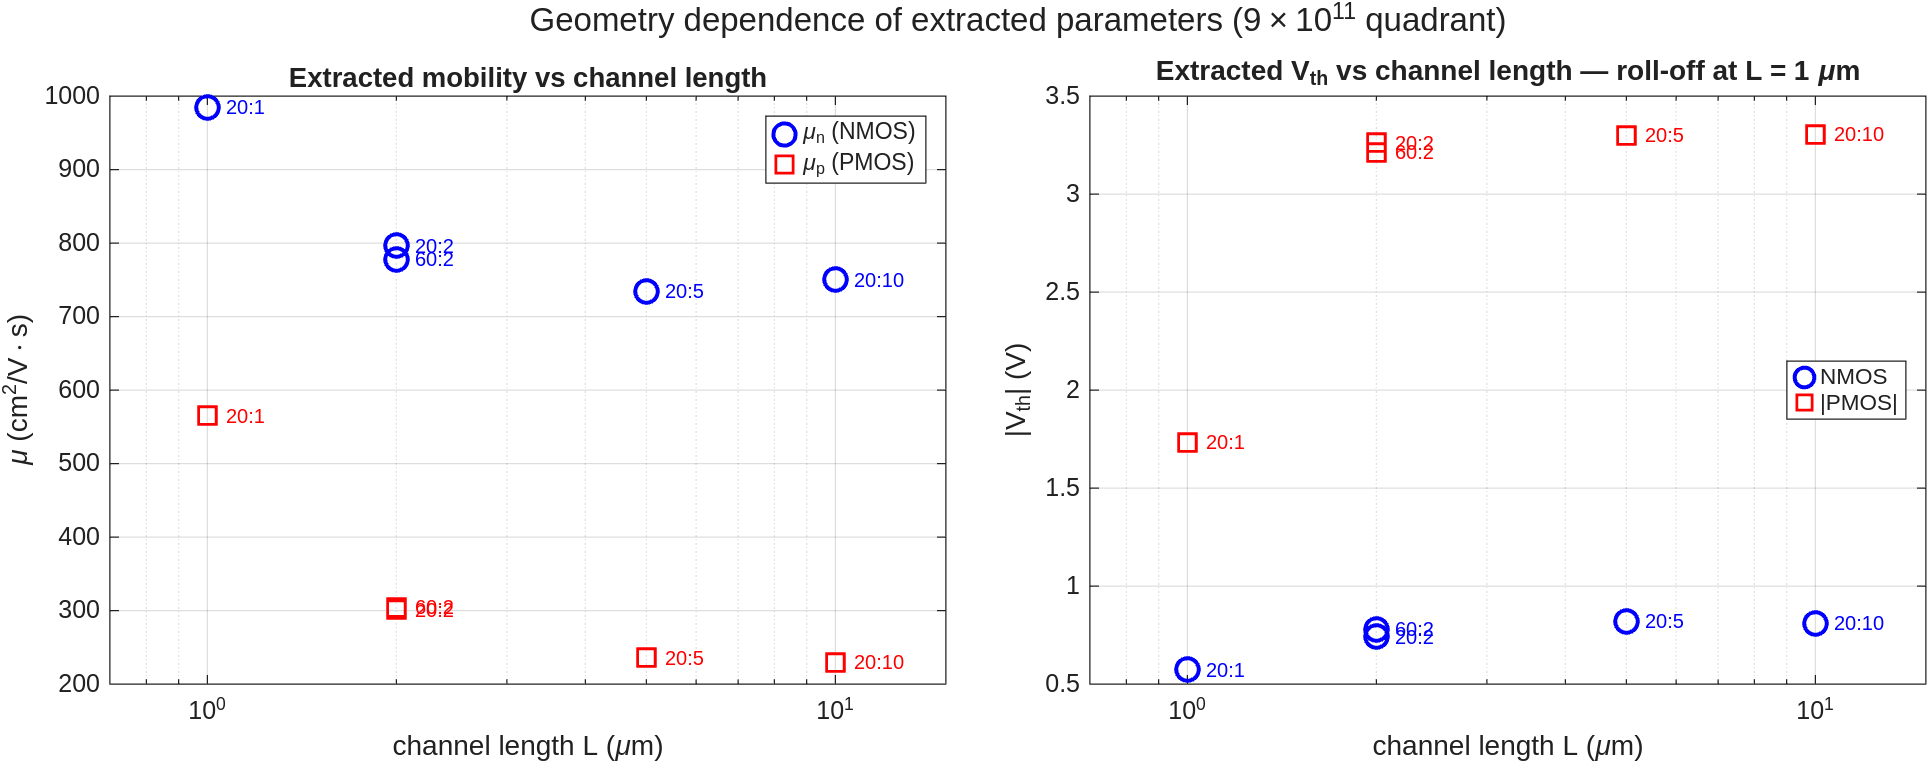
\includegraphics[width=0.9\linewidth]{Figures/mu_vth_vs_geometry.png}
  \caption{Extracted mobility and threshold voltage versus gate length. Both parameters are flat for $L \ge 2\,\mu\mathrm{m}$ and break away at $L = 1\,\mu\mathrm{m}$.}
  \label{fig:mu-vth-geom}
\end{figure}

At the shortest gate length $L = 1\,\mu\mathrm{m}$ (the $20\!:\!1$ devices), clear short-channel effects appear. The NMOS threshold voltage rolls off from about $0.82$\,V to $0.57$\,V, because the source and drain depletion regions support part of the channel depletion charge. The extracted mobility is artificially inflated ($985$ versus about $750\,\mathrm{cm}^2/\mathrm{V\,s}$), reflecting effective channel shortening and the onset of drain-induced barrier lowering (DIBL) rather than a true change in carrier transport. The PMOS suffers far more, with the threshold moving from about $-3.30$\,V to $-1.73$\,V, because its junctions are deeper ($0.59\,\mu\mathrm{m}$) and sit in the lightly doped N-Well, which makes the depletion regions wide compared to the $1\,\mu\mathrm{m}$ channel.

\subsubsection{Threshold Voltage versus $V_\mathrm{T}$-Adjust Dose}

To quantify the effect of the boron $V_\mathrm{T}$-adjust implant, the $W\!:\!L = 20\!:\!5$ transistors were measured in all four quadrants, with doses $0$, $3\times10^{11}$, $6\times10^{11}$ and $9\times10^{11}\,\mathrm{cm}^{-2}$. Figure~\ref{fig:idvg-quadrants} shows the transfer curves per quadrant, and Figure~\ref{fig:vth-dose} compares the extracted threshold voltages with the Sentaurus simulations from Section~\ref{sec:devsim}. The values are listed in Table~\ref{tab:ch6-vt-dose}.

\begin{figure}[H]
  \centering
  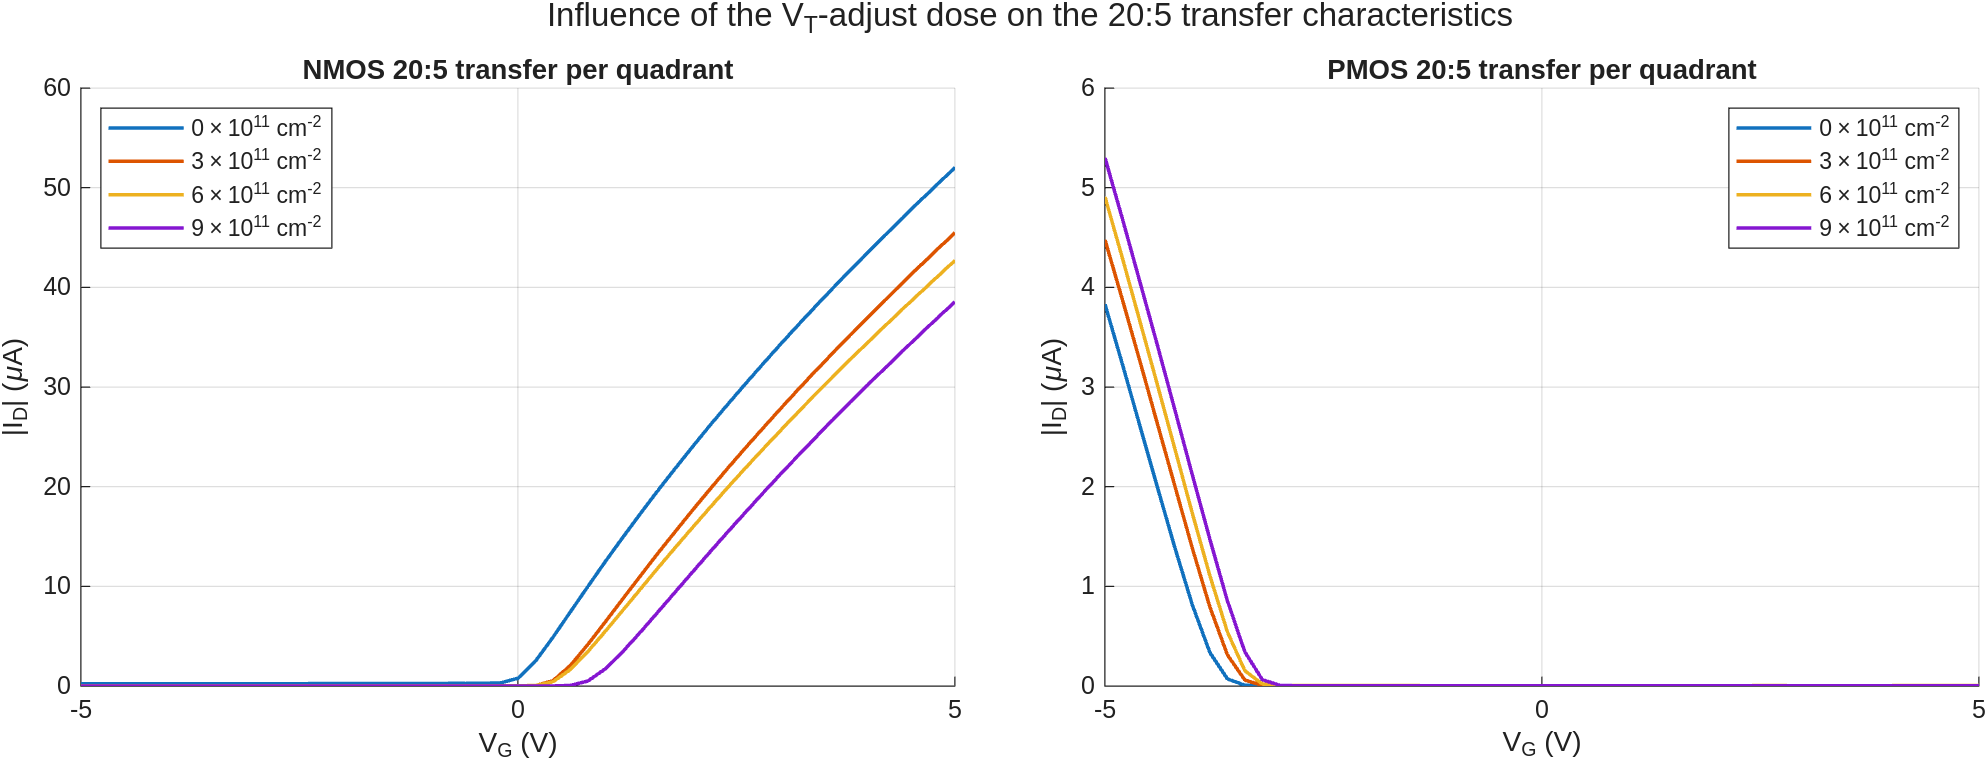
\includegraphics[width=0.95\linewidth]{Figures/idvg_quadrants.png}
  \caption{Transfer characteristics of the $20\!:\!5$ transistors in the four wafer quadrants ($V_\mathrm{T}$-adjust doses $0$ to $9\times10^{11}\,\mathrm{cm}^{-2}$).}
  \label{fig:idvg-quadrants}
\end{figure}

\begin{figure}[H]
  \centering
  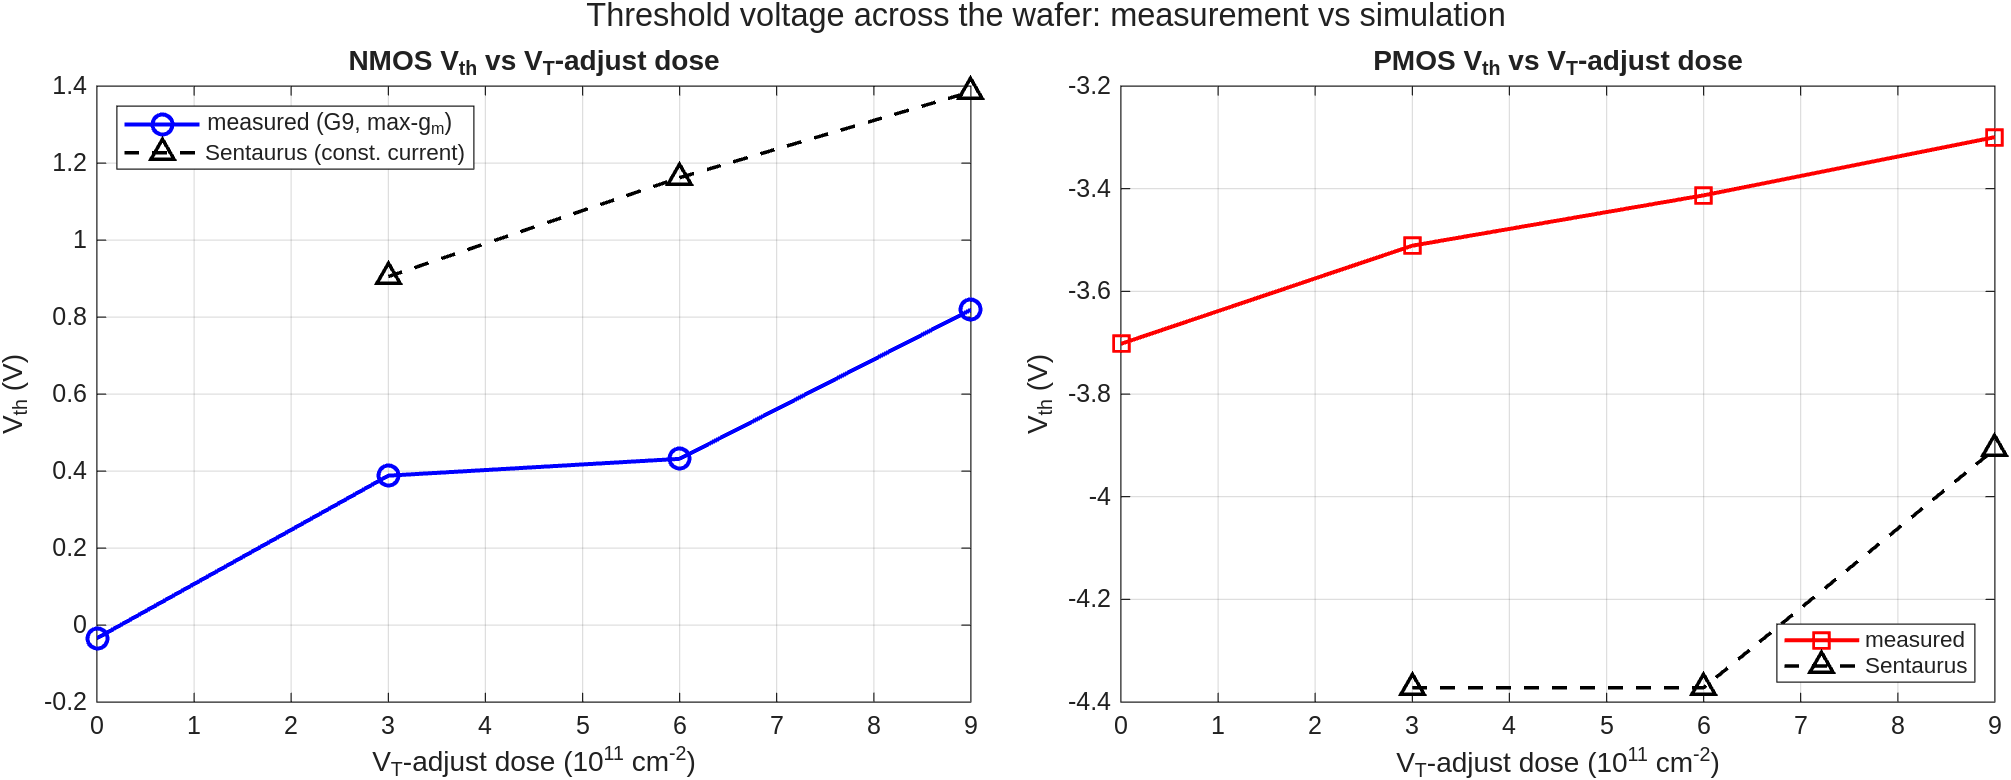
\includegraphics[width=0.95\linewidth]{Figures/vth_vs_dose.png}
  \caption{Measured threshold voltage versus $V_\mathrm{T}$-adjust dose for the $20\!:\!5$ NMOS and PMOS transistors, compared with the Sentaurus device simulations (constant-current extraction).}
  \label{fig:vth-dose}
\end{figure}

\begin{table}[htbp]
  \centering
  \caption{Threshold voltage versus $V_\mathrm{T}$-adjust dose for the $20\!:\!5$ transistors, measured and simulated (Section~\ref{sec:devsim}).}
  \label{tab:ch6-vt-dose}
  \begin{tabular}{lrrrr}
    \toprule
    Dose ($\mathrm{cm}^{-2}$) & Meas.\ $V_\mathrm{T,NMOS}$ (V) & Meas.\ $V_\mathrm{T,PMOS}$ (V) & Sim.\ $V_\mathrm{T,NMOS}$ (V) & Sim.\ $V_\mathrm{T,PMOS}$ (V) \\
    \midrule
    $0$              & -0.034 & -3.702 & --    & --    \\
    $3\times10^{11}$ &  0.388 & -3.511 & 0.905 & -4.372 \\
    $6\times10^{11}$ &  0.432 & -3.413 & 1.162 & -4.372 \\
    $9\times10^{11}$ &  0.819 & -3.300 & 1.385 & -3.907 \\
    \bottomrule
  \end{tabular}
\end{table}

The NMOS threshold voltage increases monotonically with the boron dose, from nearly $0$\,V (an almost normally-on device) to about $0.82$\,V, because the additional acceptor charge in the channel depletion region must be imaged by a larger gate voltage. The same boron implant partially compensates the N-Well surface underneath the PMOS gate, making its threshold voltage less negative by roughly $0.4$\,V over the same dose range. This is precisely the mechanism predicted by the theory in Section~\ref{sec:tech}: a single unmasked boron implant shifts both thresholds in the positive direction, which increases $|V_\mathrm{T}|$ for the NMOS and decreases it for the PMOS.

The comparison with the simulations shows the same trend and a similar dose sensitivity, but with an offset: the simulated NMOS values sit about $0.5$\,V higher and the simulated PMOS values about $0.6$\,V more negative than the measurements. Part of this offset is methodological, since the simulated values use a constant-current criterion while the measured values use maximum-transconductance extrapolation, and part is calibration, since the simulation does not include the oxide and interface charge $Q_\mathrm{ox}$ of the real gate stack, which shifts the flat-band voltage. The NMOS is roughly four times more dose-sensitive than the PMOS because the boron lands directly in its channel depletion region, whereas for the PMOS it must compete with the much higher donor concentration of the N-Well surface.

Comparing the two devices overall: the trends are the same with opposite signs, but the absolute performance differs strongly. The PMOS threshold magnitude is about four times the NMOS value, because the channel sits in the doped N-Well and the maximum applied boron dose is nowhere near enough for a symmetric pair, and the PMOS drive current and transconductance are about three times lower at equal geometry because of the lower hole mobility. A circuit designer in this process must size the PMOS about three times wider than the NMOS, and a symmetric CMOS process would need a larger $V_\mathrm{T}$-adjust dose.

\subsubsection{Output Characteristics and Channel-Length Modulation}

Output characteristics $I_\mathrm{D}(V_\mathrm{DS})$ were measured for the $20\!:\!5$ and $20\!:\!1$ devices in the $9\times10^{11}\,\mathrm{cm}^{-2}$ quadrant, with the gate voltage stepped through the linear and saturation regions ($V_\mathrm{G} = 1$ to $7$\,V for NMOS, $-1$ to $-8$\,V for PMOS). The measured families of curves are shown in Figures~\ref{fig:nmos-out} and~\ref{fig:pmos-out}. In saturation the unified model gives
\begin{equation}
  I_\mathrm{D} = \frac{\mu\, C_\mathrm{ox}}{2} \frac{W}{L} \left( V_\mathrm{GS} - V_\mathrm{T} \right)^2 \left[ 1 + \lambda \left( V_\mathrm{DS} - V_\mathrm{DS,sat} \right) \right],
  \label{eq:idsat}
\end{equation}
where $\lambda$ is the channel-length modulation parameter and $V_\mathrm{DS,sat}$ the saturation voltage. Ideally the saturation current depends only on the gate overdrive; real devices show a finite output slope.

\begin{figure}[H]
  \centering
  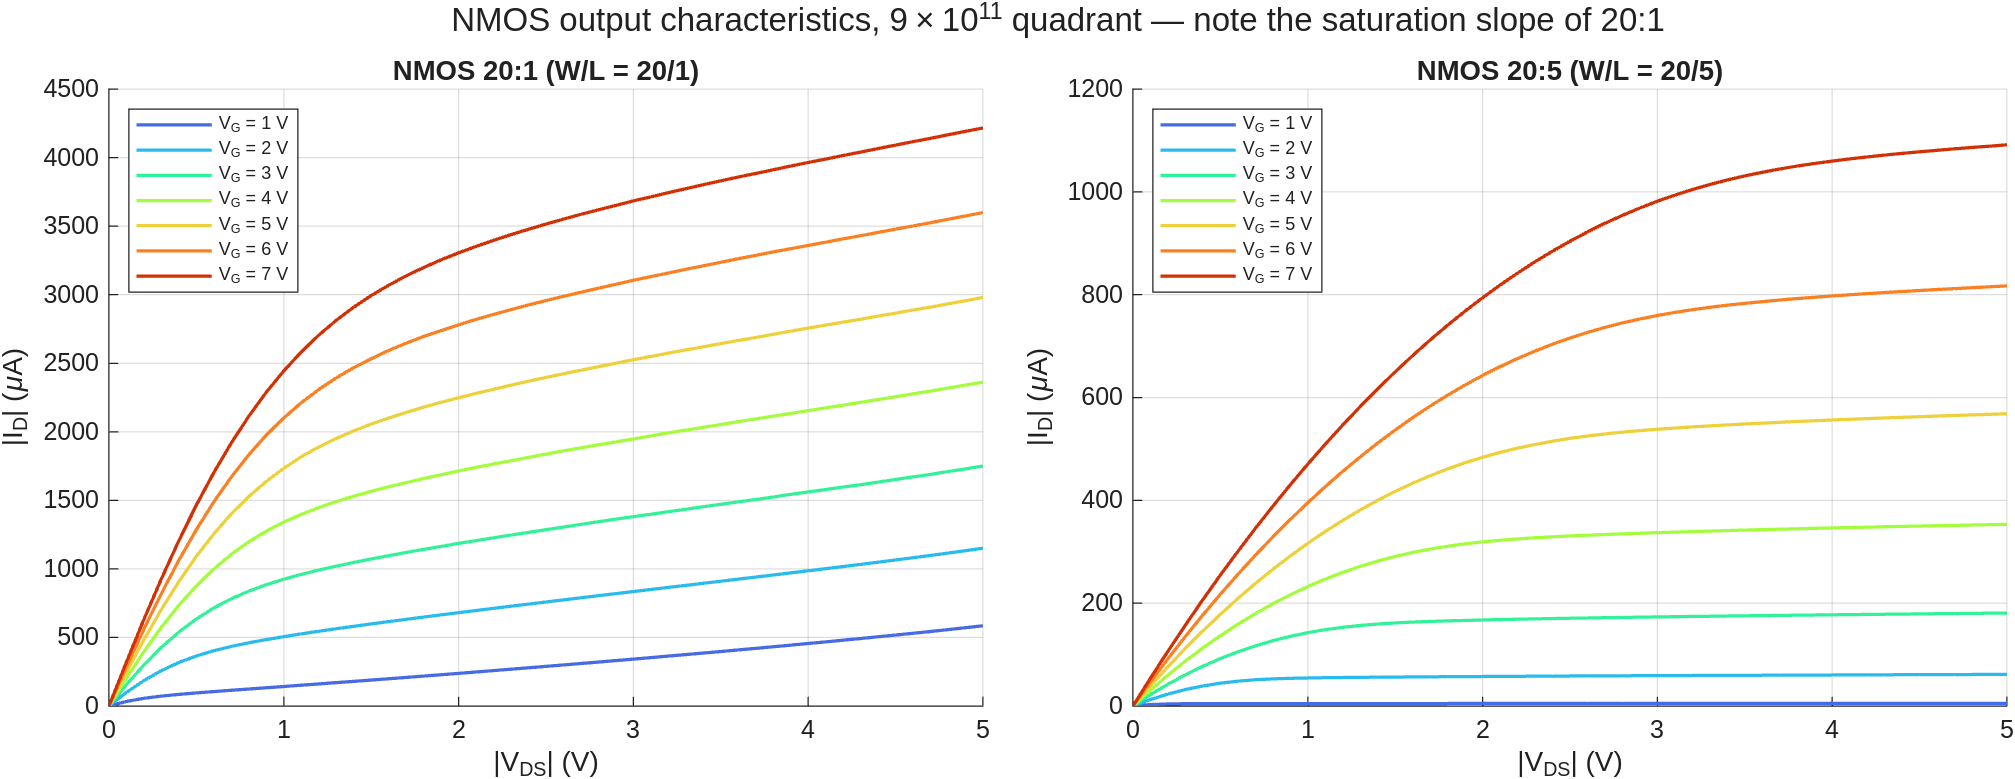
\includegraphics[width=0.95\linewidth]{Figures/nmos_idvds.png}
  \caption{Measured NMOS output characteristics for the $20\!:\!1$ and $20\!:\!5$ devices ($V_\mathrm{T}$-adjust dose $9\times10^{11}\,\mathrm{cm}^{-2}$).}
  \label{fig:nmos-out}
\end{figure}

\begin{figure}[H]
  \centering
  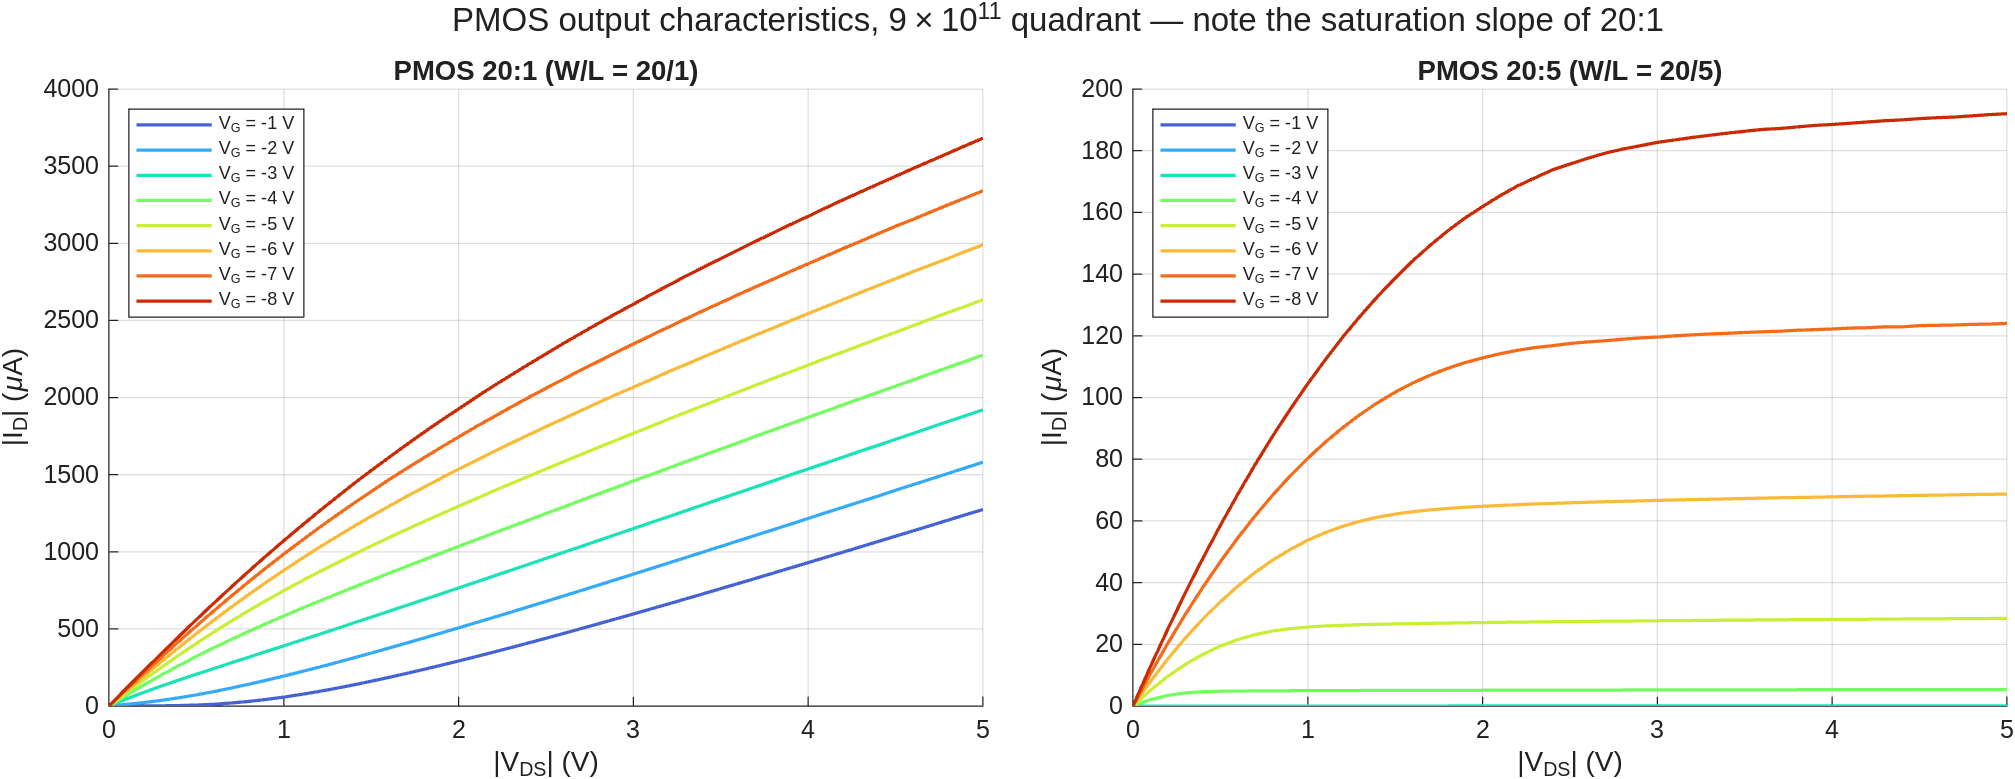
\includegraphics[width=0.95\linewidth]{Figures/pmos_idvds.png}
  \caption{Measured PMOS output characteristics for the $20\!:\!1$ and $20\!:\!5$ devices ($V_\mathrm{T}$-adjust dose $9\times10^{11}\,\mathrm{cm}^{-2}$).}
  \label{fig:pmos-out}
\end{figure}

Channel-length modulation parameters $\lambda$ were extracted from linear fits of $|I_\mathrm{D}|$ versus $|V_\mathrm{DS}|$ in the saturation region, defined as $|V_\mathrm{DS}| > |V_\mathrm{G} - V_\mathrm{T}| + 0.3$\,V. Representative values are shown in Table~\ref{tab:ch6-lambda}.

\begin{table}[htbp]
  \centering
  \caption{Channel-length modulation parameters extracted from the output characteristics.}
  \label{tab:ch6-lambda}
  \begin{tabular}{lrrl}
    \toprule
    Type & $W\!:\!L$ & $V_\mathrm{G}$ (V) & $\lambda$ ($\mathrm{V}^{-1}$) \\
    \midrule
    NMOS & 20:5 & 1 to 5   & $0.022$--$0.029$ \\
    NMOS & 20:1 & 2 to 4   & $0.16$--$0.42$ \\
    PMOS & 20:5 & $-4$ to $-7$ & $0.015$--$0.018$ \\
    PMOS & 20:1 & all  & not extractable (no true saturation) \\
    \bottomrule
  \end{tabular}
\end{table}

Besides the current magnitude, the $20\!:\!1$ and $20\!:\!5$ curves differ in shape, and two different short-channel effects are visible:

\begin{enumerate}
\item \textbf{Channel-length modulation and drain-field effects.} The pinch-off region length is set by the drain depletion width, so it consumes a fraction of the channel that scales with $1/L$. The long-channel devices show small $\lambda$ values around $0.02\,\mathrm{V}^{-1}$ and essentially flat saturation, while for the $20\!:\!1$ devices $\lambda$ is roughly an order of magnitude larger. In the extreme case the drain field reaches the source: the PMOS $20\!:\!1$ transistor never saturates within $|V_\mathrm{DS}| \le 5$\,V and behaves almost like a resistor, consistent with DIBL and the onset of punch-through. Its deep ($0.59\,\mu\mathrm{m}$) SP junctions in the lightly doped N-Well make the depletion regions as long as the drawn channel.
\item \textbf{Velocity saturation.} At $L = 1\,\mu\mathrm{m}$ the lateral field reaches the range where the carrier drift velocity saturates. Its signatures are visible in Figure~\ref{fig:idvds-norm}: the $W/L$-normalised current of the $20\!:\!1$ device falls \emph{below} that of the $20\!:\!5$ device at the same gate voltage, and successive gate-voltage curves are spaced almost linearly instead of quadratically, i.e.\ $I_\mathrm{D,sat}$ tends towards a linear dependence on $(V_\mathrm{GS}-V_\mathrm{T})$ instead of the square law of Equation~\eqref{eq:idsat}.
\end{enumerate}

\begin{figure}[H]
  \centering
  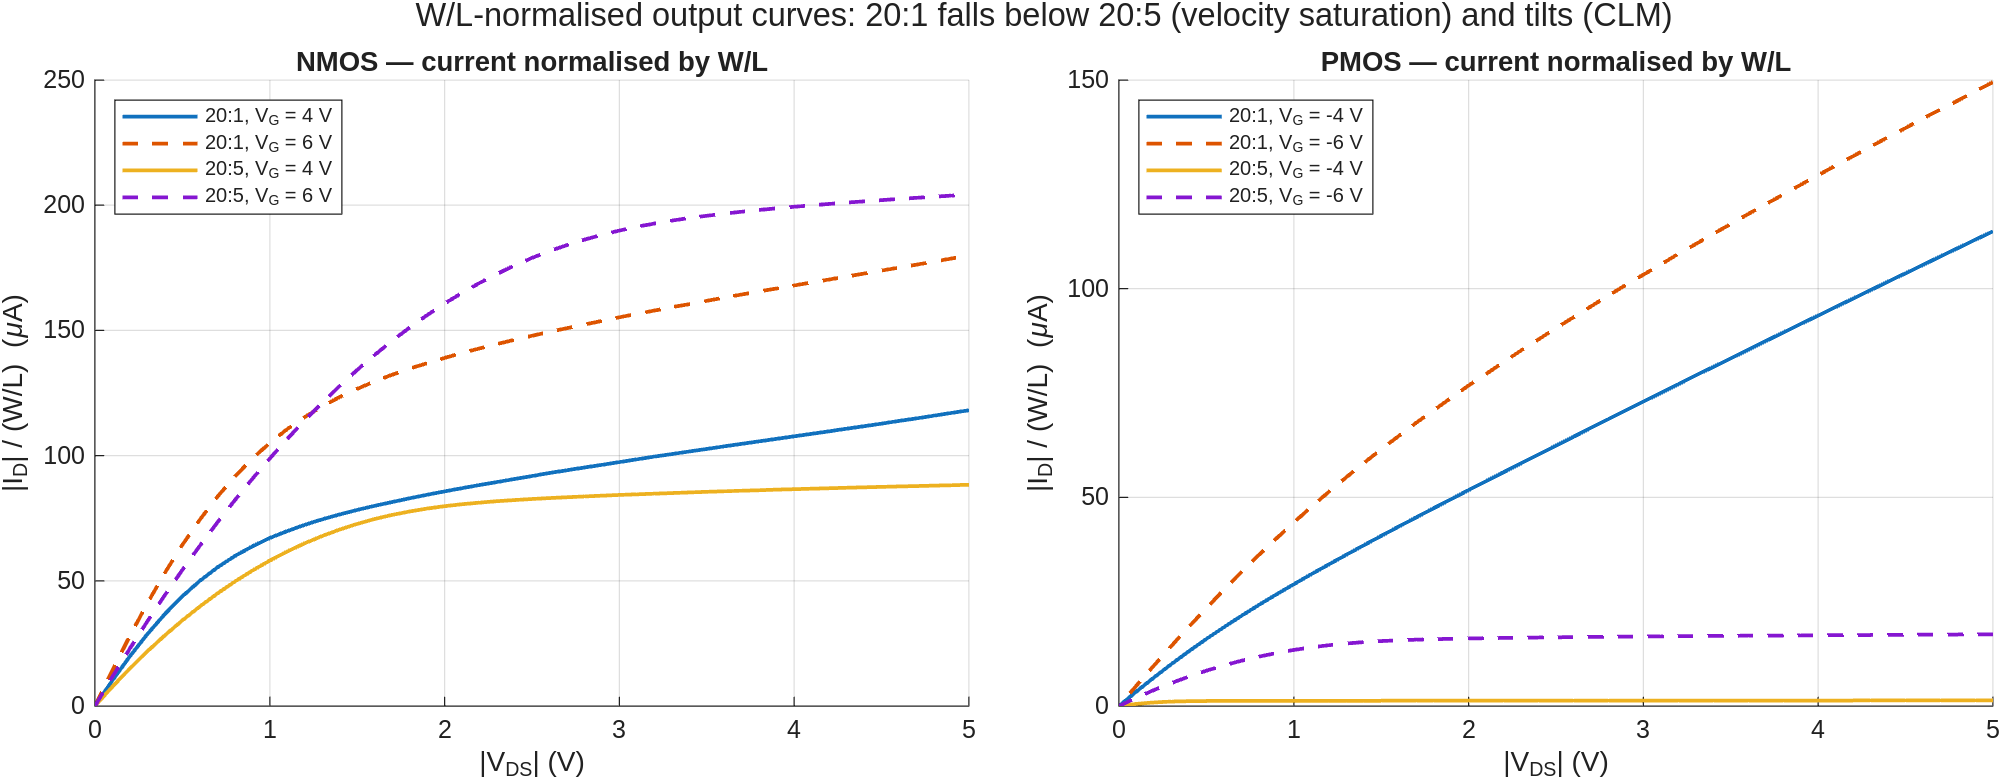
\includegraphics[width=0.95\linewidth]{Figures/idvds_normalized.png}
  \caption{$W/L$-normalised output curves of the $20\!:\!1$ and $20\!:\!5$ devices. The short-channel device carries less normalised current (velocity saturation) and its saturation region tilts (channel-length modulation); the PMOS $20\!:\!1$ device does not saturate at all.}
  \label{fig:idvds-norm}
\end{figure}

These measurements reproduce the trends seen in the Sentaurus device simulations of Section~\ref{sec:devsim}: the simulated long-channel transistors follow the square law with a small saturation slope and only a mild velocity-saturation compression at the highest gate voltages, matching our clean $20\!:\!5$ curves, while the strong short-channel degradation is only observed in the measured $L = 1\,\mu\mathrm{m}$ devices, which have no simulated counterpart. Between the two measured device types, the PMOS short-channel device degrades far more severely than the NMOS, because of its deeper junctions and the roughly ten times lower doping of the N-Well compared to the NMOS channel region.
